\documentclass{article}
\usepackage{graphicx}
\usepackage{caption}
\usepackage{float}
\usepackage[arrowdel]{physics}
\usepackage{amsmath}
\usepackage{amsfonts}
\usepackage{amsthm}
\DeclareMathOperator*{\argmax}{arg\,max}
\def\ind{\hspace{\parindent}}
\title{Report}
\author{Amirreza Negari, Amirhossein Estiri, Sajad Kahani}
\date{Augest 2019}
\begin{document}

\maketitle

\section{Optimization Problem}
let $S$ be set of feasible Hamiltonians, $\ket{\phi_0}$ the ground state and $\ket{\psi}$ the target state.

formally, problem can be formulated by this equation
\begin{equation} 
\label{eq:opt}
H^*, t^* = \argmax_{H \in S, t \in \mathbb{R}} \mathcal{F}(e^{iHt} \ket{\phi_0}, \ket{\psi})
\end{equation}

where $\mathcal{F}(., .)$ is fidelity.

\subsection{Numerical Optimization}
We can use a deep learning framework as an optimizer to solve eq. \ref{eq:opt}

We can specify the problem, for the Hamiltonian below

\begin{equation} 
\label{eq:hnearlydiag}
H = \sum_{i=1}^{\dim \mathcal{H} - 1} J_i (\dyad{i}{i + 1} + \dyad{i + 1}{i})  + \sum_{i=1}^{\dim \mathcal{H}} B_i \dyad{i}{i} 
\end{equation}

by defining $J_i$s and $B_i$s as optimization variables and then, making the computation graph of optimizing value in eq. \ref{eq:opt}, we can use gradient descent (or other optimizing methods) to solve the problem and find a value for variables although it may not be globally optimal.

This approach is the same as what Innocenti. et. al. did for gate construction. note that this method can be used for any Hamiltonian, not only eq. \ref{eq:hnearlydiag}.

here are results of applying this method on a one-sector space with aforementioned Hamiltonain, where $\ket{\phi_0} = \ket{1}$ and $\ket{\psi}$ are just random vectors.

\begin{figure}[H]
\centering
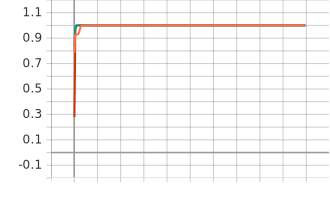
\includegraphics[width=0.4\textwidth]{fidelity_4}
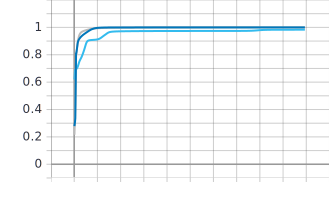
\includegraphics[width=0.4\textwidth]{fidelity_8} \\
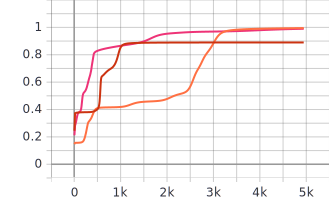
\includegraphics[width=0.4\textwidth]{fidelity_16}
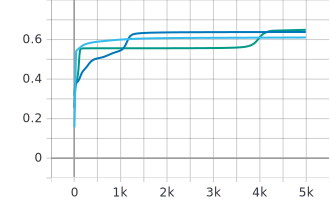
\includegraphics[width=0.4\textwidth]{fidelity_32}
\caption{fidelity vs. number of cycles for different random target vectors. 
\\ a) $\dim \mathcal{H} = 4$, b) $\dim \mathcal{H} = 8$, c) $\dim \mathcal{H} = 16$, d) $\dim \mathcal{H} = 32$
\\ Note. all of plots have the same x axis.}
\end{figure}

\subsection{Continuous Analytical Optimization}
in a continuous framework, let $\vec{v} \in \mathbb{R}^m$ degrees of freedom for the whole evolution (Hamiltonian and time).

\[ \tilde{H} = Ht = f(\vec{v}) \]
\[ \tilde{H} = \sum_{i, j} H_{ij} \dyad{i}{j} = \sum_{i, j} f_{ij}(\vec{v}) \dyad{i}{j} \]

then

\[\gradient \mathcal{F}(e^{\tilde{H}(\vec{v})} \ket{\phi_0}, \ket{\psi}) \Big|_{\vec{v} = \vec{v}^*} = \vec{0} \]

\[ \forall k \quad\quad \sum_{i,j} \pdv{\mathcal{F}(e^{iHt} \ket{\phi_0}, \ket{\psi})}{\tilde{H}_{ij}} \pdv{\tilde{H}_{ij}}{v_k}  \Big|_{\vec{v} = \vec{v}^*} = 0 \]

now we are going to compute $\pdv{\mathcal{F}}{\tilde{H}_{ij}}$

\newtheorem{lemma}{Lemma}
\begin{lemma}
\[ \pdv{H^k}{H_{mn}} = \sum_{l = 0}^{k-1} H^{l}_{mi} H^{k-l-1}_{jn} \]
\end{lemma}

\begin{lemma}
if
$H = U^\dagger D U$
\[ \pdv{H^k}{H_{mn}} = \sum_{1 \le i, j, \alpha,\beta \le \dim{\mathcal{H}}} U_{m\alpha}^\dagger U_{j\beta}^\dagger U_{\alpha i} U_{\beta n} \frac{D_{\alpha\alpha}^k - D_{\beta\beta}^k}{D_{\alpha\alpha} - D_{\beta\beta}} \dyad{i}{j} \] 
\end{lemma}

without loosing generality, we can assume $\ket{\phi_0} = \ket{1}$

by using two aformentioned lemma, we can show

\[ \begin{split} 
  \pdv{\mathcal{F}}{\tilde{H}_{ij}} = \sum_{p,q,\alpha,\beta,\gamma} \frac{\braket{\psi}{p}\braket{q}{\psi}U^\dagger_{i \alpha} U^\dagger_{1 \beta} U_{\beta j} U^\dagger_{1 \gamma}}{D_{\alpha\alpha} - D_{\beta\beta}} & ( U_{\alpha q} U_{\gamma p}(e^{iD_{\alpha\alpha}} - e^{iD_{\beta\beta}}) e^{-iD_{\gamma\gamma}} \\
   & + U_{\alpha p} U_{\gamma q} (e^{-iD_{\alpha\alpha}} - e^{-iD_{\beta\beta}}) e^{iD_{\gamma\gamma}} )
 \end{split} \]
 
 but it won't lead us to analytical solve of optimization because it needs parameteric diagonal decomposition.
\end{document}